\begin{figure*}[b]
  \centering
  \tikzstyle{large} = [circle, fill=white, text=black, draw, thick, scale=1, minimum size=0.8cm, inner sep=1.5pt]
  \tikzstyle{plain} = [circle, fill=white, text=black, draw, thick, scale=1, minimum size=0.5cm, inner sep=1.5pt]
  \tikzstyle{small} = [circle, fill=white, text=black, draw, thick, scale=1, minimum size=0.2cm, inner sep=1.5pt]
  \tikzstyle{black} = [circle, fill=gray, text=black, draw, thick, scale=1, minimum size=0.2cm, inner sep=1.5pt]
  \tikzmath{\xunit = 0.8; \yunit = 0.8;}

  \begin{minipage}[m]{.48\textwidth}
      \vspace{0pt}
      \centering
      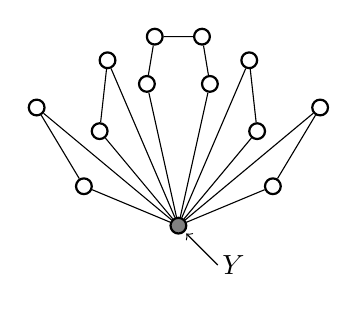
\begin{tikzpicture}
          % vertices
          \node[black] (y1) at (0, 0) {};
          \node[small] (a1) at (-1.2, 0.5) {};
          \node[small] (a2) at (-1.8, 1.5) {};
          \node[small] (b1) at (-1.0, 1.2) {};
          \node[small] (b2) at (-0.9, 2.1) {};
          \node[small] (c1) at (-0.4, 1.8) {};
          \node[small] (c2) at (-0.3, 2.4) {};
          \node[small] (c3) at (0.3, 2.4) {};
          \node[small] (c4) at (0.4, 1.8) {};
          \node[small] (d1) at (1.0, 1.2) {};
          \node[small] (d2) at (0.9, 2.1) {};
          \node[small] (e1) at (1.2, 0.5) {};
          \node[small] (e2) at (1.8, 1.5) {};

          %edges
          \draw (y1)--(a1)--(a2)--(y1);
          \draw (y1)--(b1)--(b2)--(y1);
          \draw (y1)--(c1)--(c2)--(c3)--(c4)--(y1);
          \draw (y1)--(d1)--(d2)--(y1);
          \draw (y1)--(e1)--(e2)--(y1);
          

          \node[] at (0.7, -0.5) {$Y$};
          \draw[->] (0.5,-0.5)--(0.1,-0.1);
      \end{tikzpicture}
  \end{minipage}
  %
  \hfill
  %
  \begin{minipage}[m]{.48\textwidth}
    \vspace{0pt}
    \centering
    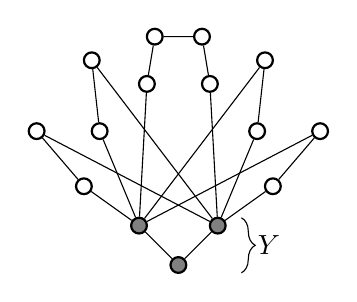
\begin{tikzpicture}
        % vertices
        \node[black] (y1) at (0, -0.5) {};
        \node[black] (y2) at (-0.5, 0) {};
        \node[black] (y3) at (0.5, 0) {};
        \node[small] (a1) at (-1.2, 0.5) {};
        \node[small] (a2) at (-1.8, 1.2) {};
        \node[small] (b1) at (-1.0, 1.2) {};
        \node[small] (b2) at (-1.1, 2.1) {};
        \node[small] (c1) at (-0.4, 1.8) {};
        \node[small] (c2) at (-0.3, 2.4) {};
        \node[small] (c3) at (0.3, 2.4) {};
        \node[small] (c4) at (0.4, 1.8) {};
        \node[small] (d1) at (1.0, 1.2) {};
        \node[small] (d2) at (1.1, 2.1) {};
        \node[small] (e1) at (1.2, 0.5) {};
        \node[small] (e2) at (1.8, 1.2) {};

        %edges
        \draw (y2)--(y1)--(y3);
        \draw (y2)--(a1)--(a2)--(y3);
        \draw (y2)--(b1)--(b2)--(y3);
        \draw (y2)--(c1)--(c2)--(c3)--(c4)--(y3);
        \draw (y2)--(d2)--(d1)--(y3);
        \draw (y2)--(e2)--(e1)--(y3);

        \draw [decorate,decoration={brace,amplitude=5pt}]
        (0.8, 0.1) -- (0.8, -0.6) node[midway,xshift=10pt]{$Y$};
    \end{tikzpicture}
\end{minipage}
%
% \hfill
% %
% \begin{minipage}[m]{.40\textwidth}
%   \vspace{0pt}
%   \centering
%   \begin{tikzpicture}
%     \draw (0, 2 * \yunit) rectangle (3 * \xunit, 0);
%     \draw (1 * \xunit, 0) -- (1 * \xunit, 2 * \yunit);
%     \draw (1 * \xunit, 1 * \yunit) -- (3 * \xunit, 1 * \yunit);
%     \draw (0, 3.4 * \yunit) rectangle (3 * \xunit, 2.4 * \yunit);
%     \draw (0.5 * \xunit, 2 * \yunit) -- (0.5 * \xunit, 2.4 * \yunit);
%     \draw (2 * \xunit, 2 * \yunit) -- (2 * \xunit, 2.4 * \yunit);
%     \draw (5.5 * \xunit, 2 * \yunit) rectangle (6.2 * \xunit, 0 * \yunit);

%     \node[] at (0.5 * \xunit, 0.4 * \yunit) {$X$};
%     \node[] at (2 * \xunit, 1.5 * \yunit) {$Y$};
%     \node[] at (2 * \xunit, 0.5 * \yunit) {$Z$};
%     \node[] at (1.5 * \xunit, 2.9 * \yunit) {$B$};

%     \draw[dashed,rounded corners] (-0.1 * \xunit, 2.1 * \yunit) rectangle (3.2 * \xunit, 0.9 * \yunit);
%     \draw[dashed,rounded corners] (-0.2 * \xunit, 2.2 * \yunit) rectangle (6.3 * \xunit, 0.8 * \yunit);
%     \draw[dashed,rounded corners] (-0.3 * \xunit, 3.6 * \yunit) rectangle (4 * \xunit, -0.2 * \yunit);
%     \draw[dashed,rounded corners] (-0.4 * \xunit, 3.7 * \yunit) rectangle (6.5 * \xunit, -0.3 * \yunit);
%     \node[] at (3.6 * \xunit, 1.5 * \yunit) {$X_C'$};
%     \node[] at (4.4 * \xunit, 3.2 * \yunit) {$H'$};
%     \node[] at (6.2 * \xunit, 3.4 * \yunit) {$H$};
%     \node[] at (5.4 * \xunit, 2.5 * \yunit) {$X_C$};
%     \node[] at (4.8 * \xunit, 1.6 * \yunit) {\huge $\dots$};
%   \end{tikzpicture}
% \end{minipage}
%
  \caption{%
  Examples of odd cycle sunflowers of order $5$ with core $Y$.
  The union of the core and each petal induces an odd cycle.
  % The left two figures (left, middle) show examples of odd cycle sunflowers of order $5$ with core $Y$.
  %
  % The right figure shows a construction used in the proof of \Cref{lem:redundant-component}.
  % $H'$ is a component in $H'$, and $H'[B]$ is a component in $H'-X_C$, where $X_C$ is an OCT of $H$.
  % $X$ is also an OCT of $H'-B$, and by definition $H'[B]$ and $H'[Y \cup Z]$ are bipartite.
  }
  \label{fig:proof-component}
\end{figure*}
